\documentclass[english]{report}
\usepackage[english]{babel} 
\usepackage[T1]{fontenc}
\usepackage[utf8]{inputenc}
\usepackage{float}
\usepackage{graphicx}

\makeatletter
\usepackage[a4paper,top=2cm,bottom=2cm,left=2cm,right=2cm]{geometry}
\usepackage{enumitem}
\usepackage{subfig}
\usepackage{amsthm}
\usepackage{amsmath}
\usepackage{epstopdf}
\usepackage{fancyhdr}
\usepackage{booktabs,array}
\usepackage{tabularx}
\usepackage{hyperref}
\hypersetup{
    colorlinks=true,
    linkcolor=blue,
    filecolor=magenta,      
    urlcolor=cyan,
    citecolor=blue
}

\hyphenation{english}
\makeatother

\usepackage{listings}
\usepackage{xcolor} % for setting colors

% set the default code style
\lstset{
    frame=tb, % draw a frame at the top and bottom of the code block
    tabsize=4, % tab space width
    showstringspaces=false, % don't mark spaces in strings
    numbers=left, % display line numbers on the left
    commentstyle=\color{gray}, % comment color
    keywordstyle=\color{blue}, % keyword color
    stringstyle=\color{red} % string color
}


\begin{document}
\begin{titlepage}

	\begin{center}
		\begin{Large} \textbf{UNIVERSITY OF PADOVA} \\
		\end{Large} \vspace{1cm}
		\vspace{3cm}
		\begin{Large} Embedded Real--Time Control \end{Large}
		\par\end{center}

	\begin{center}
		\begin{Large}Laboratory report\\
		\end{Large}
		\par\end{center}

	\begin{center}
		\vspace{2cm}
		\begin{figure}[!htb]
			\centering 
\includegraphics[width=8cm]{figures/unipd-logo.png}\\

		\end{figure}

		\par\end{center}

	\begin{center}
		\vspace{2cm}
		\begin{Large} Names - (Student ID Numbers)  \\
		\end{Large} \vspace{2cm}
		\begin{Large} Academic Year 2021-2022 \end{Large}
		\par\end{center}

\end{titlepage}

\tableofcontents
\newpage

% Chapters inclusion
\chapter{Laboratory 1: \texorpdfstring{$\text{I}^2\text{C}$}{I2C} Peripheral Integration -- Line Sensor and Matrix Keypad}
\label{chap:lab1}

\section{Introduction and Objectives}
In embedded real-time systems, microcontrollers must continuously interact with the external physical environment through sensors and with human operators through input/output peripherals. However, directly dedicating microcontroller General Purpose Input/Output (GPIO) pins to every individual sensing element or button quickly exhausts the available pin count, reduces board layout flexibility, and impairs deterministic real-time execution. To overcome these constraints, serial communication buses such as $\text{I}^2\text{C}$ (Inter-Integrated Circuit) are widely employed to multiplex dozens of digital signals onto a shared two-wire interface.

The primary objective of Laboratory 1 is to achieve hands-on proficiency in low-level peripheral communication using the $\text{I}^2\text{C}$ protocol on an ARM Cortex-M7 based STM32F7 microcontroller platform. The experimental hardware consists of a mobile robot rover (Figure~\ref{fig:turtlebot_platform}) equipped with two Semtech SX1509 16-channel $\text{I}^2\text{C}$ GPIO expanders sharing the primary hardware bus (\texttt{I2C1}):
\begin{itemize}[noitemsep,topsep=3pt]
    \item \textbf{Device 1 (\texttt{SX1509\_1}, 7-bit slave address \texttt{0x3E}):} Interfaces with an 8-element Pololu QTR Reflectance Sensor array positioned beneath the front section of the rover to detect road markings and line boundaries.
    \item \textbf{Device 2 (\texttt{SX1509\_2}, 7-bit slave address \texttt{0x3F}):} Operates as an autonomous matrix keypad engine scanning a $4 \times 4$ tactile switch keypad (16 keys) and asserting an active-low external interrupt line (\texttt{NINT}) routed to pin \texttt{PF4} on the STM32F7.
\end{itemize}

\begin{figure}[htbp]
    \centering
    \fbox{
        \begin{minipage}{0.88\textwidth}
            \vspace{8pt}
            \centering
            \textbf{[FIGURE PLACEHOLDER: Mobile Robot Experimental Setup]} \\[6pt]
            \begin{flushleft}
            \footnotesize
            \textbf{Target file:} \texttt{figures/turtlebot\_platform.png} (or existing \texttt{figures/turtlebot\_1.jpg}) \\
            \textbf{Description:} Photograph showing the mobile robot rover platform used in the laboratory. \\
            \textbf{Key elements to display:}
            \begin{itemize}[noitemsep,topsep=2pt]
                \item STM32F7 microcontroller board mounted on the main chassis.
                \item Underside front bracket mounting the Pololu QTR 8-channel reflectance array.
                \item $4 \times 4$ tactile matrix keypad mounted on the upper deck for user interaction.
                \item Shared $\text{I}^2\text{C}$ ribbon cable wiring and power distribution.
            \end{itemize}
            \textit{Note: Reference photographs of the platform are already present at \texttt{Report/figures/turtlebot\_1.jpg}.}
            \end{flushleft}
            \vspace{4pt}
        \end{minipage}
    }
    %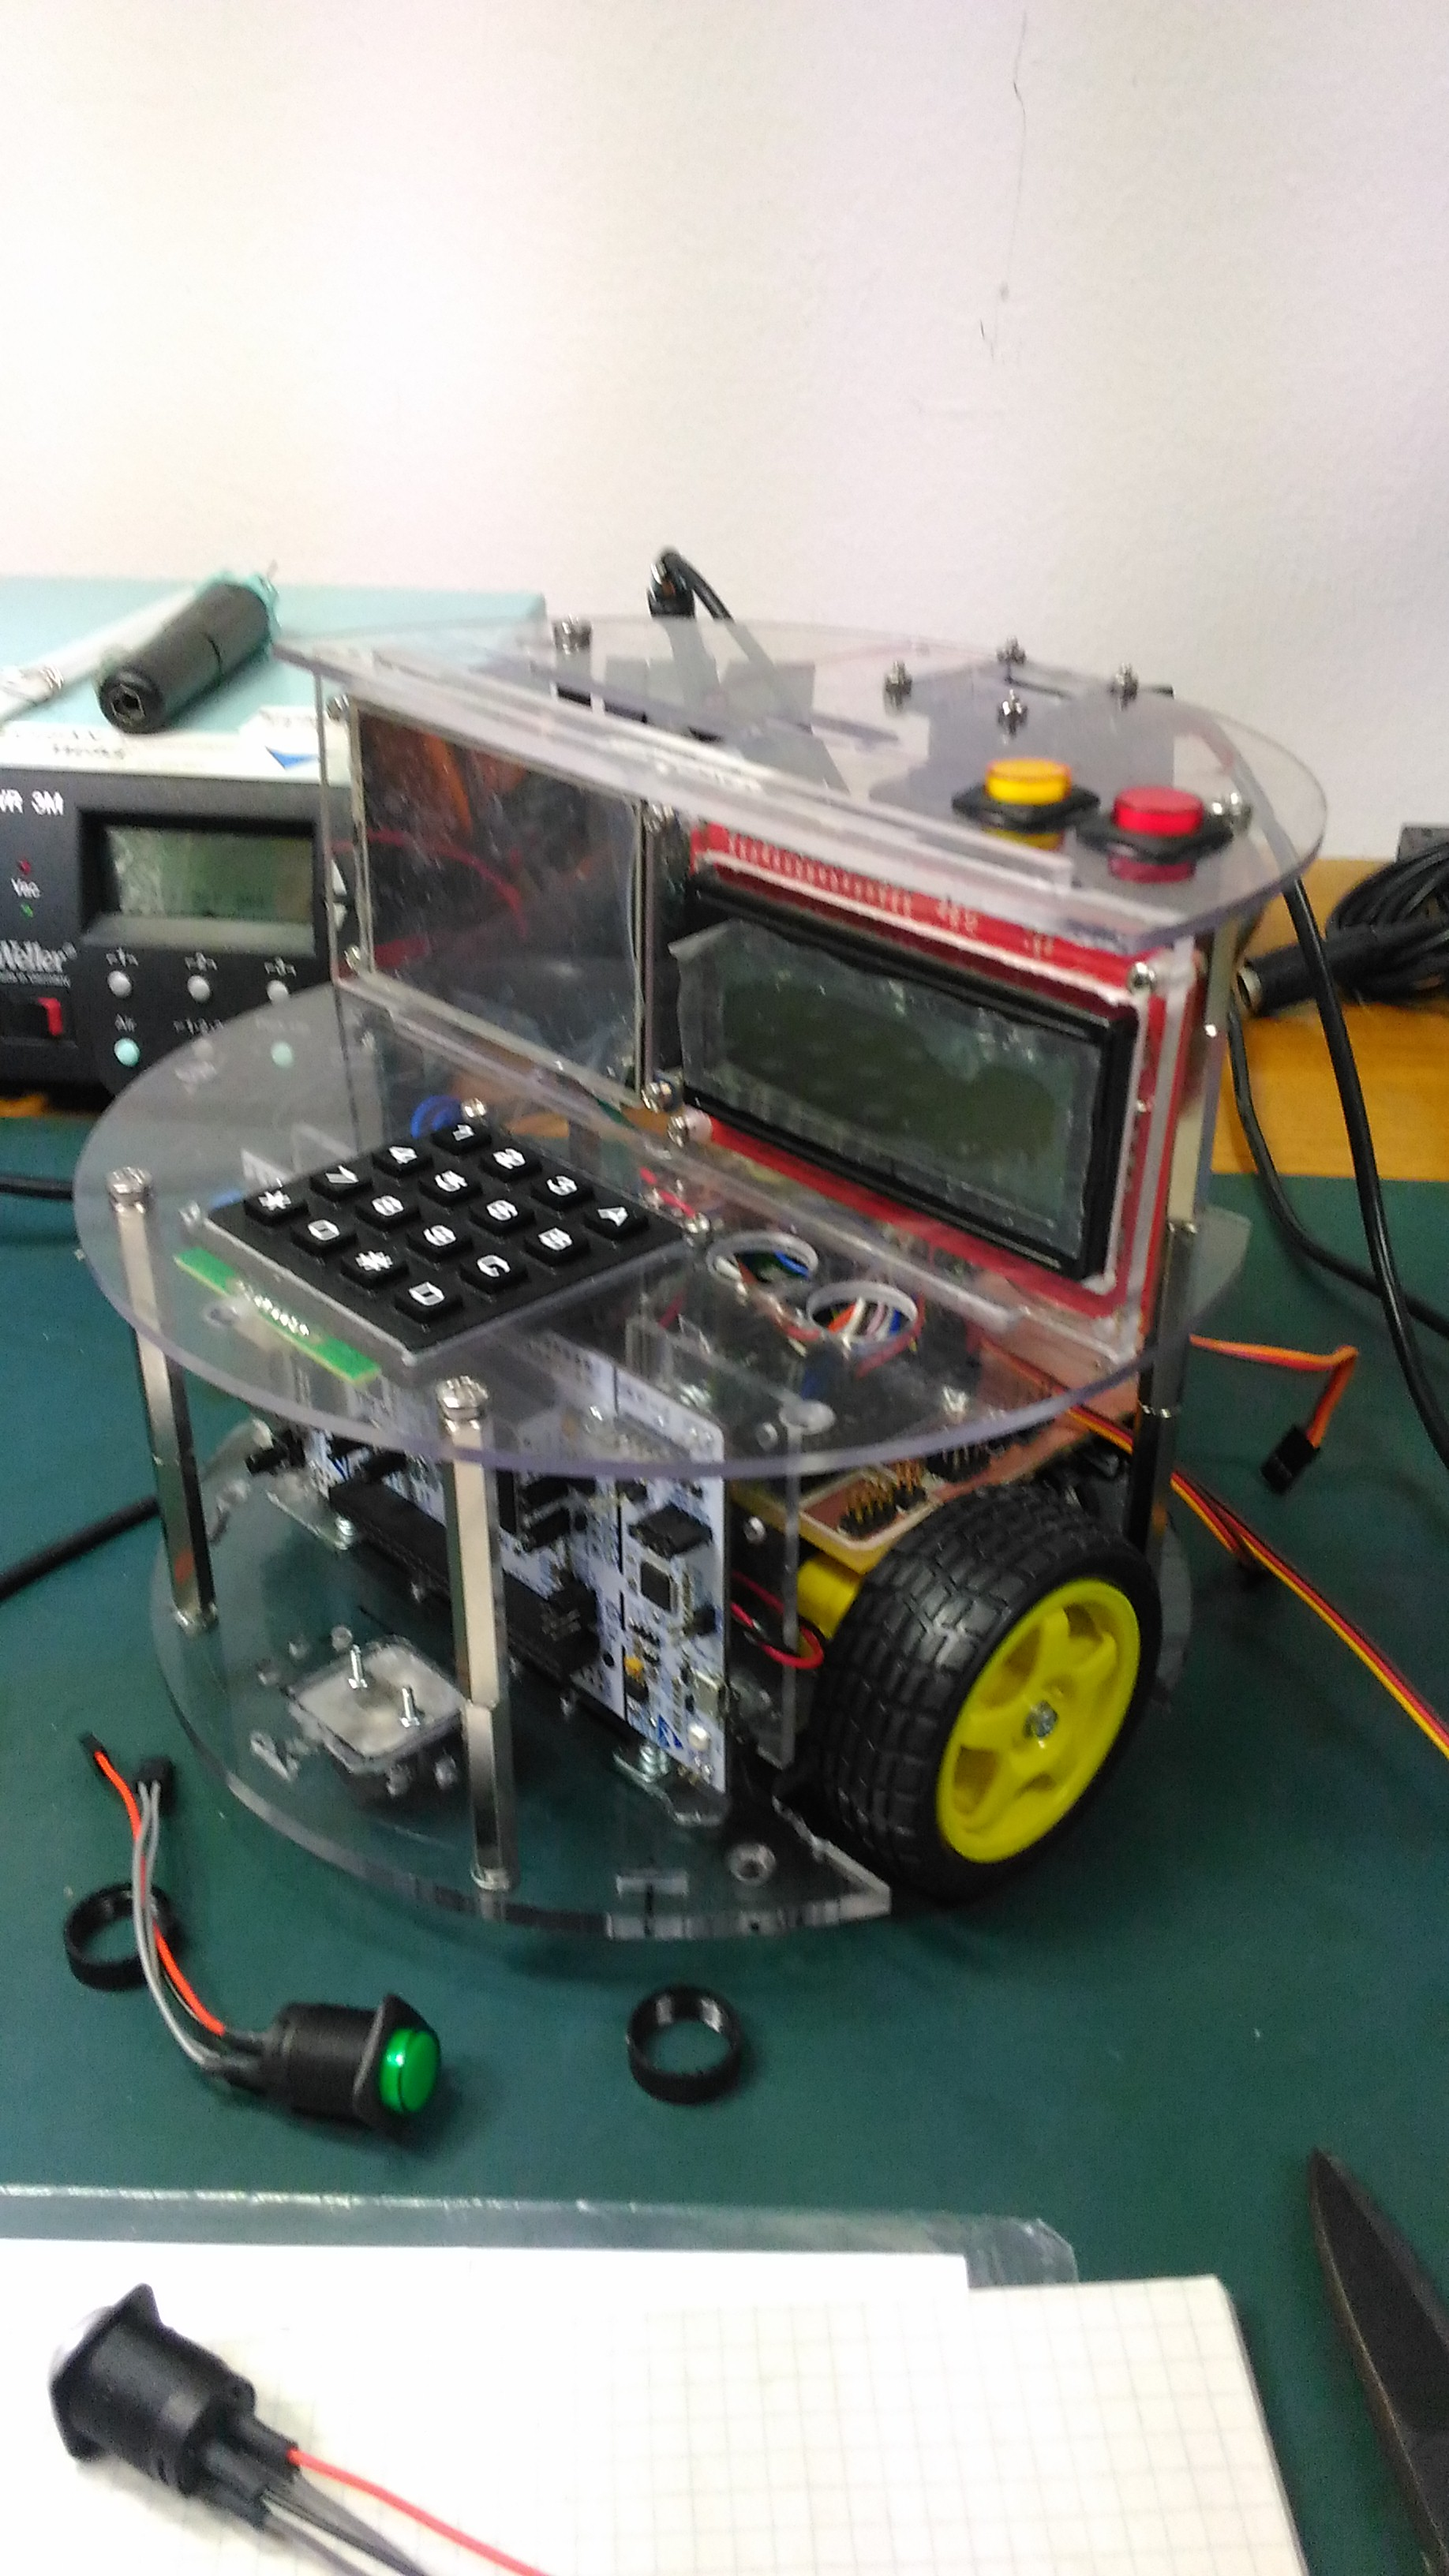
\includegraphics[width=0.55\textwidth]{figures/turtlebot_1.jpg}
    \caption{The TurtleBot mobile robot rover platform equipped with the STM32F7 core, underside optical line sensor array, and top-mounted matrix keypad.}
    \label{fig:turtlebot_platform}
\end{figure}

The laboratory activity is structured into five sequential exercises:
\begin{enumerate}[noitemsep,topsep=3pt]
    \item \textbf{Exercise 1 -- External Interrupt Service Routine (ISR):} Implementing the EXTI callback for pin \texttt{PF4} to detect keypresses and performing the required register read sequence on \texttt{SX1509\_2} to de-assert the interrupt latch.
    \item \textbf{Exercise 2 -- Keypad Matrix Decoding:} Decoding raw column and row bitmask values into matrix coordinates and resolving the pressed alphanumeric characters via a 2D lookup table calibrated against physical rover routing.
    \item \textbf{Exercise 3 -- Line Sensor Polling:} Designing a periodic polling routine in the main execution thread to sample the 8-bit line sensor bitmask with a nominal period of $100\text{ ms}$.
    \item \textbf{Exercise 4 -- Timer-Driven Non-Blocking Sampling:} Replacing software polling with hardware timer \texttt{TIM6} update interrupts, configuring prescaler and auto-reload values to achieve deterministic $10\text{ Hz}$ non-blocking telemetry.
    \item \textbf{Exercise 5 -- Dynamic Frequency Actuation:} Modulating the blinking frequency of an external LED on pin \texttt{PE5} through keypad inputs, evaluating both direct static key-to-frequency mapping and dynamic multi-digit ASCII string parsing with execute delimiters.
\end{enumerate}

Real-time diagnostic telemetry and register outputs were monitored using the ARM CoreSight Single Wire Output (SWO) Instrumentation Trace Macrocell (ITM), redirected through a custom implementation of the low-level \texttt{\_write()} system call.

\section{Problem Analysis and Design Decisions}

\subsection{Pin Conservation and Serial Bus Multiplexing}
Direct interfacing of the onboard peripherals would impose significant hardware overhead: the 8-element Pololu QTR line sensor requires 8 digital inputs, while the $4 \times 4$ matrix keypad demands 4 output drive lines and 4 input sensing lines, totaling 16 dedicated GPIO pins. On a microcontroller driving dual DC motors, quadrature encoder feedback channels, display interfaces, and communication peripherals, reserving 16 high-speed pins for static I/O is unsustainable.

Offloading these peripherals to dual Semtech SX1509 expanders collapses the pin requirement down to three physical connections: the serial clock line (\texttt{SCL}), the serial data line (\texttt{SDA}), and a single shared external interrupt line (\texttt{NINT} to \texttt{PF4}). 

However, sharing a half-duplex serial bus introduces critical design trade-offs:
\begin{itemize}[noitemsep,topsep=2pt]
    \item \textbf{Bus Contention and Addressing:} Multiple slaves cannot transmit simultaneously. Collision avoidance is guaranteed by unique 7-bit addressing (\texttt{0x3E} for \texttt{SX1509\_1} and \texttt{0x3F} for \texttt{SX1509\_2}).
    \item \textbf{Addressing Bit Shift in STM32 HAL:} The STM32 Hardware Abstraction Layer (HAL) expects the device address byte pre-shifted to the left by 1 bit, reserving the Least Significant Bit (LSB) for the Read/$\overline{\text{Write}}$ flag:
    \begin{equation}
        \text{DevAddress}_{\text{HAL}} = (\text{Address}_{\text{7-bit}} \ll 1) \mid \text{R}/\overline{\text{W}}
    \end{equation}
    Consequently, \texttt{SX1509\_1} (\texttt{0x3E}) becomes \texttt{0x7C}, and \texttt{SX1509\_2} (\texttt{0x3F}) becomes \texttt{0x7E}. Omitting this shift is a frequent source of communication failure.
\end{itemize}

\subsection{Asynchronous Input vs. Periodic Telemetry}
The two peripherals exhibit contrasting operational dynamics:
\begin{enumerate}[noitemsep,topsep=2pt]
    \item \textbf{Keypad (Sporadic, Asynchronous):} User keypresses occur unpredictably and last between $50\text{ ms}$ and $300\text{ ms}$. Polling the keypad inside a loop is inefficient: if the loop period is too slow, brief keypresses are missed; if too fast, the CPU wastes cycles in busy-wait polling. Utilizing the hardware interrupt line (\texttt{NINT}) on \texttt{PF4} ensures instant response with zero background CPU overhead.
    \item \textbf{Line Sensor (Continuous, Synchronous):} Ground line tracking requires steady, deterministic feedback at fixed sampling intervals. While polling with software delays (\texttt{HAL\_Delay()}) functions in isolation, it completely stalls CPU execution, introducing timing jitter and blocking other control loops. A hardware timer interrupt (\texttt{TIM6}) provides strictly periodic execution without blocking the foreground thread.
\end{enumerate}

\subsection{Interrupt Latching and Deadlock Prevention}
A crucial architectural feature of the SX1509 keypad engine is its internal interrupt latch. When a key is actuated, the open-drain \texttt{NINT} line transitions to logic low and remains asserted until both the column register (\texttt{REG\_KEY\_DATA\_1}, \texttt{0x27}) and the row register (\texttt{REG\_KEY\_DATA\_2}, \texttt{0x28}) are fully read by the host over $\text{I}^2\text{C}$. If the microcontroller acknowledges the EXTI interrupt without executing these read transactions, the physical line remains at $0\text{ V}$, preventing subsequent falling edges and causing permanent input deadlock.

\section{Relevant Theoretical Background and System Architecture}

\subsection{\texorpdfstring{$\text{I}^2\text{C}$}{I2C} Bus Topology and Communication Protocol}
The $\text{I}^2\text{C}$ protocol is a synchronous, multi-master, multi-slave, packet-switched serial bus developed by Philips Semiconductor. As illustrated in Figure~\ref{fig:i2c_architecture}, the physical interface relies on two bidirectional open-drain lines pulled up to $V_{\text{DD}} = 3.3\text{ V}$ via external resistors ($R_P \approx 4.7\text{ k}\Omega$):
\begin{itemize}[noitemsep,topsep=2pt]
    \item \textbf{SCL (Serial Clock Line):} Generated by the bus master (STM32F7) to synchronize data bit transitions.
    \item \textbf{SDA (Serial Data Line):} Carries serialized data bytes, sampled during the high phase of SCL and modified during the low phase.
\end{itemize}

\begin{figure}[htbp]
    \centering
    \fbox{
        \begin{minipage}{0.88\textwidth}
            \vspace{8pt}
            \centering
            \textbf{[FIGURE PLACEHOLDER: I2C Hardware Topology Diagram]} \\[6pt]
            \begin{flushleft}
            \footnotesize
            \textbf{Target file:} \texttt{figures/i2c\_architecture.png} \\
            \textbf{Description:} Comprehensive schematic block diagram of the $\text{I}^2\text{C}1$ serial bus interconnects. \\
            \textbf{Key elements to display:}
            \begin{itemize}[noitemsep,topsep=2pt]
                \item STM32F7 microcontroller acting as Master, showing \texttt{I2C1\_SCL} and \texttt{I2C1\_SDA} pins.
                \item Pull-up resistors ($4.7\text{ k}\Omega$) connecting SCL and SDA to $V_{\text{DD}} = 3.3\text{ V}$.
                \item \texttt{SX1509\_1} slave block (7-bit address \texttt{0x3E}) connected to the 8 IR reflectance sensor pins.
                \item \texttt{SX1509\_2} slave block (7-bit address \texttt{0x3F}) connected to the $4 \times 4$ matrix keypad.
                \item Dedicated active-low interrupt line \texttt{NINT} running from \texttt{SX1509\_2} to STM32 pin \texttt{PF4}.
                \item Visual distinction between serial bus lines (shared) and point-to-point interrupt line.
            \end{itemize}
            \end{flushleft}
            \vspace{4pt}
        \end{minipage}
    }
    %\includegraphics[width=0.85\textwidth]{figures/i2c_architecture.png}
    \caption{Hardware interconnect diagram of the $\text{I}^2\text{C}1$ bus, detailing master-slave relationships, peripheral addresses, pull-up terminations, and the dedicated \texttt{PF4} interrupt line.}
    \label{fig:i2c_architecture}
\end{figure}

Communication frames adhere to strict signaling rules:
\begin{itemize}[noitemsep,topsep=2pt]
    \item \textbf{START Condition ($S$):} A high-to-low transition on SDA while SCL is high.
    \item \textbf{Address Frame:} 7 bits of slave address transmitted MSB first, followed by the eighth bit specifying data direction ($0 = \text{Write}$, $1 = \text{Read}$).
    \item \textbf{Acknowledge (ACK / NACK):} The receiving device pulls SDA low during the ninth clock cycle to signal successful byte reception (ACK) or leaves it high (NACK).
    \item \textbf{STOP Condition ($P$):} A low-to-high transition on SDA while SCL is high, relinquishing the bus.
\end{itemize}

\subsection{Pololu QTR Reflectance Sensor Array}
The Pololu QTR reflectance array consists of $N = 8$ optical sensing elements arranged in a linear array with constant spacing (pitch) $P = 8\text{ mm} = 0.008\text{ m}$, as depicted in Figure~\ref{fig:line_sensor_geometry}.

\begin{figure}[htbp]
    \centering
    \fbox{
        \begin{minipage}{0.88\textwidth}
            \vspace{8pt}
            \centering
            \textbf{[FIGURE PLACEHOLDER: Line Sensor Physical Geometry and Array Spacing]} \\[6pt]
            \begin{flushleft}
            \footnotesize
            \textbf{Target file:} \texttt{figures/line\_sensor\_geometry.png} \\
            \textbf{Description:} Schematic diagram detailing the mechanical arrangement and geometric pitch of the 8-element Pololu QTR array. \\
            \textbf{Key elements to display:}
            \begin{itemize}[noitemsep,topsep=2pt]
                \item Array of 8 sensing elements indexed from 0 (leftmost) to 7 (rightmost).
                \item Dimension callout showing constant pitch $P = 8\text{ mm}$ between element centers.
                \item Overall array sensing width $W = (N - 1) \cdot P = 56\text{ mm}$.
                \item Rover geometric centerline marking the zero reference position ($x = 0\text{ mm}$).
                \item Inset diagram showing infrared LED emitter and phototransistor pair reflection off white vs. black surface.
            \end{itemize}
            \end{flushleft}
            \vspace{4pt}
        \end{minipage}
    }
    %\includegraphics[width=0.75\textwidth]{figures/line_sensor_geometry.png}
    \caption{Geometrical layout of the Pololu QTR 8-element optical reflectance sensor array showing indexing convention, element pitch ($P = 8\text{ mm}$), and center line reference.}
    \label{fig:line_sensor_geometry}
\end{figure}

Each sensing element pairs an infrared Light Emitting Diode ($\lambda \approx 940\text{ nm}$) with an NPN silicon phototransistor:
\begin{itemize}[noitemsep,topsep=2pt]
    \item \textbf{White Background (High Reflectance):} Infrared photons bounce off the light surface into the phototransistor base, driving it into full saturation. The output node is pulled to ground, yielding a logical \texttt{0}.
    \item \textbf{Black Guidance Line (High Absorption):} Carbon-black pigment absorbs infrared radiation. The phototransistor remains cut off, and an internal pull-up drives the output high, yielding a logical \texttt{1}.
\end{itemize}

The states of all eight sensing channels are latched into Bank B of \texttt{SX1509\_1} in register \texttt{REG\_DATA\_B} (address \texttt{0x10}). Reading this single 8-bit register retrieves the full spatial state as an integer bitmask:
\begin{equation}
    D_{\text{byte}} = \sum_{i=0}^{7} b_i \cdot 2^i, \quad b_i \in \{0, 1\}
\end{equation}
where bit $b_i$ represents the binary state of sensing element $i$ (with $b_0$ as LSB). For example, if the black trajectory line covers elements 3 and 4:
\begin{equation}
    D_{\text{byte}} = 2^3 + 2^4 = 8 + 16 = 24 = \texttt{0x18} = (00011000)_2
\end{equation}

In subsequent closed-loop control laboratories (Laboratory 4), this bitmask is converted into a physical position error $x_{\text{line}}$ relative to the rover center using a weighted centroid formula:
\begin{equation}
    x_i = \left(i - \frac{N - 1}{2}\right) \cdot P = (i - 3.5) \cdot 8\text{ mm}
\end{equation}
\begin{equation}
    x_{\text{line}} = \frac{\sum_{i=0}^{7} b_i \cdot x_i}{\sum_{i=0}^{7} b_i}
    \label{eq:centroid}
\end{equation}

\subsection{Matrix Keypad Engine and Interrupt Generation}
The keypad is constructed as a $4 \times 4$ mechanical switch matrix. Rather than requiring continuous software scanning, \texttt{SX1509\_2} incorporates a dedicated hardware keypad engine. The 4 column lines and 4 row lines are connected to internal weak pull-up resistors, maintaining an idle logic high level ($1$) across all pins.

\begin{figure}[htbp]
    \centering
    \fbox{
        \begin{minipage}{0.88\textwidth}
            \vspace{8pt}
            \centering
            \textbf{[FIGURE PLACEHOLDER: Matrix Keypad Circuit Schematic]} \\[6pt]
            \begin{flushleft}
            \footnotesize
            \textbf{Target file:} \texttt{figures/keypad\_schematic.png} \\
            \textbf{Description:} Electrical schematic of the $4 \times 4$ matrix keypad connected to \texttt{SX1509\_2}. \\
            \textbf{Key elements to display:}
            \begin{itemize}[noitemsep,topsep=2pt]
                \item Matrix grid with 4 row lines (\texttt{Row0}--\texttt{Row3}) and 4 column lines (\texttt{Col0}--\texttt{Col3}).
                \item 16 tactile push buttons positioned at grid intersections.
                \item Internal pull-up resistors inside the SX1509 tied to $V_{\text{DD}}$.
                \item Example current path highlighted when button \texttt{'8'} or button \texttt{'4'} is depressed, driving specific row/column lines to ground.
                \item Corresponding register bit assignments for \texttt{REG\_KEY\_DATA\_1} and \texttt{REG\_KEY\_DATA\_2}.
            \end{itemize}
            \end{flushleft}
            \vspace{4pt}
        \end{minipage}
    }
    %\includegraphics[width=0.55\textwidth]{figures/keypad_schematic.png}
    \caption{Schematic of the $4 \times 4$ switch matrix connected to \texttt{SX1509\_2}, illustrating the pull-up configuration and active-low ground path established upon key depression.}
    \label{fig:keypad_schematic}
\end{figure}

The SX1509 engine cycles through the columns and reads the rows. In the unpressed idle state, reading the column status register \texttt{REG\_KEY\_DATA\_1} (\texttt{0x27}) and row status register \texttt{REG\_KEY\_DATA\_2} (\texttt{0x28}) yields \texttt{0xFF} ($255$). When a key is pressed, mechanical contact bridges the corresponding row and column, pulling the respective bit lines low ($0$).

Upon detecting a valid keypress, the SX1509 triggers the active-low open-drain \texttt{NINT} output line, pulling pin \texttt{PF4} of the STM32 to ground. The line remains low until both \texttt{REG\_KEY\_DATA\_1} and \texttt{REG\_KEY\_DATA\_2} are retrieved by the host microcontroller over $\text{I}^2\text{C}$.

\subsection{STM32 Nested Vectored Interrupt Controller and EXTI Architecture}
The STM32F7 Nested Vectored Interrupt Controller (NVIC) manages peripheral interrupt priorities and execution vectors. External GPIO pin events are handled by the External Interrupt/Event Controller (EXTI). Pin \texttt{PF4} is multiplexed onto EXTI Line 4. The EXTI edge-detection block was configured for \textit{Falling Edge Trigger Mode} with internal pull-up and pull-down resistors disabled (relying on the external pull-up of the open-drain \texttt{NINT} line).

When a falling edge occurs on \texttt{PF4}, the NVIC executes \texttt{EXTI4\_IRQHandler()}, triggering the HAL dispatch routine:
\begin{center}
\texttt{HAL\_GPIO\_EXTI\_IRQHandler(GPIO\_PIN\_4)}
\end{center}
This function clears the EXTI pending bit in hardware and executes the weak-aliased user callback:
\begin{lstlisting}[language=C]
void HAL_GPIO_EXTI_Callback(uint16_t GPIO_Pin);
\end{lstlisting}
Crucially, the parameter \texttt{GPIO\_Pin} passed to this callback is the pin bitmask (\texttt{GPIO\_PIN\_4} $= \texttt{0x0010} = 16$), rather than the scalar index $4$.

\subsection{Hardware Timer Architecture and Non-Blocking Scheduling}
To eliminate busy-waiting in line sensor acquisition, basic timer \texttt{TIM6} was employed. \texttt{TIM6} consists of a 16-bit auto-reload upcounter driven by the internal APB1 peripheral timer clock ($f_{\text{TIM\_CLK}}$). The update event frequency $f_{\text{INT}}$ is governed by the 16-bit Prescaler (\texttt{PSC}) and Auto-Reload Register (\texttt{ARR}):
\begin{equation}
    f_{\text{INT}} = \frac{f_{\text{TIM\_CLK}}}{(\text{PSC} + 1) \cdot (\text{ARR} + 1)}
    \label{eq:timer_freq}
\end{equation}
When the counter overflows from \texttt{ARR} back to 0, an update interrupt is generated, dispatching:
\begin{lstlisting}[language=C]
void HAL_TIM_PeriodElapsedCallback(TIM_HandleTypeDef *htim);
\end{lstlisting}
This allows execution of periodic transactions in the background while leaving the main loop unblocked.

\subsection{Instrumentation Trace Macrocell (ITM) Debug Telemetry}
Standard embedded implementations of \texttt{printf()} frequently route output over a UART port, which introduces substantial blocking delays at standard baud rates (e.g., $115200\text{ bps} \approx 87\ \mu\text{s}$ per character). On ARM Cortex-M7 cores, the Single Wire Viewer (SWV) utilizes the Instrumentation Trace Macrocell (ITM) hardware trace port. Characters written to ITM Stimulus Port 0 are serialized by dedicated CoreSight hardware over the SWO pin at high core frequencies without stalling the CPU pipeline.

To redirect standard C output stream to SWV, the low-level system call \texttt{\_write()} was implemented:
\begin{lstlisting}[language=C, caption={Low-level standard output redirection to ITM Stimulus Port 0.}, label={lst:write_redirect}]
int _write(int file, char *ptr, int len)
{
    int DataIdx;
    for (DataIdx = 0; DataIdx < len; DataIdx++)
    {
        ITM_SendChar(*ptr++);
    }
    return len;
}
\end{lstlisting}

\section{Code Structure and Implementation Choices}

\subsection{Development Environment and Diagnostic Toolchain}
The implementation and testing of Laboratory 1 relied on a professional embedded engineering toolchain:
\begin{itemize}[noitemsep,topsep=2pt]
    \item \textbf{STM32CubeIDE (v1.8+):} The primary integrated development environment based on Eclipse, providing the GNU ARM Embedded Toolchain (\texttt{arm-none-eabi-gcc}), automated build pipelines, and GDB-based debugging support.
    \item \textbf{STM32CubeMX:} Graphical peripheral and clock tree configuration tool. Used to configure PLL clock multipliers ($f_{\text{SYSCLK}} = 96\text{ MHz}$, $f_{\text{PCLK1}} = 48\text{ MHz}$), pin multiplexing (setting \texttt{PF4} as external falling-edge interrupt and \texttt{PE5} as push-pull output), and initializing \texttt{TIM6} basic timer parameters.
    \item \textbf{Serial Wire Viewer (SWV) ITM Data Console:} Hardware trace utility embedded within ARM CoreSight debug infrastructure. Enabled via Stimulus Port 0 to display high-speed real-time \texttt{printf()} diagnostic telemetry without imposing intrusive UART transmission delays.
    \item \textbf{Digital Oscilloscope / Logic Analyzer:} Utilized to verify physical pin states, capturing the falling edges on \texttt{PF4} generated by the SX1509 expander, inspecting $\text{I}^2\text{C}$ clock/data handshakes, and measuring the modulated output frequency on LED pin \texttt{PE5}.
\end{itemize}

\subsection{Software Architecture Overview}
The software architecture was designed to cleanly separate hardware initialization, asynchronous interrupt handling, deterministic periodic sampling, and foreground user-interface logic. The complete application source code is divided across two reference implementations in the repository:
\begin{itemize}[noitemsep,topsep=2pt]
    \item \texttt{lab1/c/lab1\_es123.c}: Covers Exercises 1, 2, and 3 (keypad interrupt handling, coordinate decoding, and line sensor polling).
    \item \texttt{lab1/c/lab1\_es45.c}: Covers Exercises 4 and 5 (timer-driven \texttt{TIM6} line sensor acquisition and dynamic LED frequency modulation).
\end{itemize}

\subsection{Exercise 1: Keypad Interrupt Service Routine and Register Re-arming}
In Exercise 1, the external interrupt callback \texttt{HAL\_GPIO\_EXTI\_Callback} was implemented to intercept keypress events on pin \texttt{PF4}. As described in Section~\ref{chap:lab1}, the SX1509 \texttt{NINT} pin is latched low upon key actuation. To de-assert this hardware line and prepare the peripheral for subsequent events, both \texttt{REG\_KEY\_DATA\_1} (\texttt{0x27}) and \texttt{REG\_KEY\_DATA\_2} (\texttt{0x28}) must be read over $\text{I}^2\text{C}$ inside the callback.

\begin{lstlisting}[language=C, caption={EXTI callback handling keypad interrupt and clearing SX1509 latch.}, label={lst:ex1_isr}]
uint8_t data_col;
uint8_t data_row;

void HAL_GPIO_EXTI_Callback(uint16_t GPIO_Pin)
{
    printf("Interrupt on pin (%d).\n", GPIO_Pin);

    if (GPIO_Pin == GPIO_PIN_4)
    {
        /* Read column status register (REG_KEY_DATA_1, 0x27) */
        HAL_I2C_Mem_Read(&hi2c1,
                         SX1509_I2C_ADDR2 << 1,
                         REG_KEY_DATA_1,
                         1,
                         &data_col,
                         1,
                         I2C_TIMEOUT);

        /* Read row status register (REG_KEY_DATA_2, 0x28) */
        HAL_I2C_Mem_Read(&hi2c1,
                         SX1509_I2C_ADDR2 << 1,
                         REG_KEY_DATA_2,
                         1,
                         &data_row,
                         1,
                         I2C_TIMEOUT);

        printf("REG_KEY_DATA_1: %u | REG_KEY_DATA_2: %u\n", data_col, data_row);
    }
}
\end{lstlisting}

\textbf{Implementation Observation on Pin Bitmask:} Inspection of the console output revealed that \texttt{printf("Interrupt on pin (\%d)", GPIO\_Pin)} printed the integer value \texttt{16}. In the STM32 HAL library, \texttt{GPIO\_PIN\_4} is defined as a bitmask:
\begin{equation}
    \texttt{GPIO\_PIN\_4} = ((uint16\_t)0x0010) = 16
\end{equation}
The conditional check \texttt{if (GPIO\_Pin == GPIO\_PIN\_4)} correctly matches this value.

\subsection{Exercise 2: Key Code Decoding and Matrix Calibration}
Exercise 2 requires translating the raw register byte values (\texttt{data\_col} and \texttt{data\_row}) into matrix row and column indices ($0$ to $3$), and resolving the pressed alphanumeric key.

\subsubsection{Bitmask-to-Index Decoding Implementation Choice}
Because the SX1509 active-low lines pull exactly one bit to ground per single keypress, the active register states correspond to:
\begin{itemize}[noitemsep,topsep=2pt]
    \item Bit 0 low ($2^0$ pulled down): $255 - 1 = 254 = \texttt{0xFE}$
    \item Bit 1 low ($2^1$ pulled down): $255 - 2 = 253 = \texttt{0xFD}$
    \item Bit 2 low ($2^2$ pulled down): $255 - 4 = 251 = \texttt{0xFB}$
    \item Bit 3 low ($2^3$ pulled down): $255 - 8 = 247 = \texttt{0xF7}$
\end{itemize}

To map these four values to coordinate indices $0, 1, 2, 3$, a \texttt{switch-case} construct was chosen over nested \texttt{if-else} branches or logarithmic arithmetic. Under GCC ARM optimization, switch-case constructs over small, contiguous integer ranges compile into jump tables or single conditional branch instructions, delivering deterministic, sub-microsecond execution inside the ISR.

\begin{lstlisting}[language=C, caption={Coordinate decoding and lookup table evaluation.}, label={lst:ex2_decode}]
uint8_t col = 0, row = 0;

switch (data_col) {
    case 254: col = 0; break;
    case 253: col = 1; break;
    case 251: col = 2; break;
    case 247: col = 3; break;
}

switch (data_row) {
    case 254: row = 0; break;
    case 253: row = 1; break;
    case 251: row = 2; break;
    case 247: row = 3; break;
}

printf("col: %d, row: %d\n", col, row);
printf("pressed key: %c\n", keypadLayout[row][col]);
\end{lstlisting}

\subsubsection{Hardware Matrix Discrepancy and Layout Calibration}
During experimental testing, an important discrepancy between the course theoretical handouts and the physical hardware was uncovered. In the theoretical handout schematic, the primary diagonal of equal coordinates was described as running from key \texttt{'1'} ($254, 254$) down to key \texttt{'D'} ($247, 247$). 

However, systematically pressing each physical key on the rover and observing the raw SWV console logs revealed that:
\begin{itemize}[noitemsep,topsep=2pt]
    \item Key \texttt{'*'} generated \texttt{REG\_KEY\_DATA\_1 = 254} and \texttt{REG\_KEY\_DATA\_2 = 254} (coordinates $0, 0$).
    \item Key \texttt{'A'} generated \texttt{REG\_KEY\_DATA\_1 = 247} and \texttt{REG\_KEY\_DATA\_2 = 247} (coordinates $3, 3$).
\end{itemize}
The matrix row lines on the physical rover were routed in reverse vertical order compared to the theoretical diagram. To account for this hardware reality without adding software computational overhead, the 2D character lookup matrix was calibrated as follows:

\begin{lstlisting}[language=C, caption={Calibrated keypad layout matrix matching physical hardware wiring.}, label={lst:keypad_layout}]
const char keypadLayout[4][4] = {
    {'*', '0', '#', 'D'},   /* Row 0 (REG_KEY_DATA_2 = 254) */
    {'7', '8', '9', 'C'},   /* Row 1 (REG_KEY_DATA_2 = 253) */
    {'4', '5', '6', 'B'},   /* Row 2 (REG_KEY_DATA_2 = 251) */
    {'1', '2', '3', 'A'}    /* Row 3 (REG_KEY_DATA_2 = 247) */
};
/* Columns:
   Col 0 (254): '*', '7', '4', '1'
   Col 1 (253): '0', '8', '5', '2'
   Col 2 (251): '#', '9', '6', '3'
   Col 3 (247): 'D', 'C', 'B', 'A' */
\end{lstlisting}

Table~\ref{tab:keypad_truth_table} summarizes the complete decoding truth table verified experimentally on the hardware.

\begin{table}[htbp]
    \centering
    \small
    \caption{Keypad Matrix Register Decoding Truth Table experimentally verified on the rover.}
    \label{tab:keypad_truth_table}
    \begin{tabular}{cccccc}
        \toprule
        \textbf{Key} & \textbf{Col Reg (\texttt{0x27})} & \textbf{Row Reg (\texttt{0x28})} & \textbf{Col ($c$)} & \textbf{Row ($r$)} & \textbf{Dec Pair ($d_1, d_2$)} \\
        \midrule
        \texttt{*} & \texttt{0xFE} / 254 & \texttt{0xFE} / 254 & 0 & 0 & (254, 254) \\
        \texttt{0} & \texttt{0xFD} / 253 & \texttt{0xFE} / 254 & 1 & 0 & (253, 254) \\
        \texttt{\#} & \texttt{0xFB} / 251 & \texttt{0xFE} / 254 & 2 & 0 & (251, 254) \\
        \texttt{D} & \texttt{0xF7} / 247 & \texttt{0xFE} / 254 & 3 & 0 & (247, 254) \\
        \midrule
        \texttt{7} & \texttt{0xFE} / 254 & \texttt{0xFD} / 253 & 0 & 1 & (254, 253) \\
        \texttt{8} & \texttt{0xFD} / 253 & \texttt{0xFD} / 253 & 1 & 1 & (253, 253) \\
        \texttt{9} & \texttt{0xFB} / 251 & \texttt{0xFD} / 253 & 2 & 1 & (251, 253) \\
        \texttt{C} & \texttt{0xF7} / 247 & \texttt{0xFD} / 253 & 3 & 1 & (247, 253) \\
        \midrule
        \texttt{4} & \texttt{0xFE} / 254 & \texttt{0xFB} / 251 & 0 & 2 & (254, 251) \\
        \texttt{5} & \texttt{0xFD} / 253 & \texttt{0xFB} / 251 & 1 & 2 & (253, 251) \\
        \texttt{6} & \texttt{0xFB} / 251 & \texttt{0xFB} / 251 & 2 & 2 & (251, 251) \\
        \texttt{B} & \texttt{0xF7} / 247 & \texttt{0xFB} / 251 & 3 & 2 & (247, 251) \\
        \midrule
        \texttt{1} & \texttt{0xFE} / 254 & \texttt{0xF7} / 247 & 0 & 3 & (254, 247) \\
        \texttt{2} & \texttt{0xFD} / 253 & \texttt{0xF7} / 247 & 1 & 3 & (253, 247) \\
        \texttt{3} & \texttt{0xFB} / 251 & \texttt{0xF7} / 247 & 2 & 3 & (251, 247) \\
        \texttt{A} & \texttt{0xF7} / 247 & \texttt{0xF7} / 247 & 3 & 3 & (247, 247) \\
        \bottomrule
    \end{tabular}
\end{table}

\subsection{Exercise 3: Line Sensor Polling Implementation}
In Exercise 3, a synchronous polling routine was written in the main thread to sample the line sensor state every $100\text{ ms}$.

\begin{lstlisting}[language=C, caption={Synchronous polling of the Pololu QTR line sensor in main().}, label={lst:ex3_polling}]
uint8_t data_line;
HAL_StatusTypeDef status;

while (1)
{
    status = HAL_I2C_Mem_Read(&hi2c1,
                             SX1509_I2C_ADDR1 << 1,
                             REG_DATA_B,
                             1,
                             &data_line,
                             1,
                             I2C_TIMEOUT);

    if (status != HAL_OK)
        printf("I2C communication error (%X).\n", status);
    else
        printf("Data line: %d\n", data_line);

    HAL_Delay(100);
}
\end{lstlisting}

\textbf{Critique of Software Polling:} While straightforward, this pattern is unsuited for real-time control. \texttt{HAL\_Delay(100)} executes a blocking loop monitoring the SysTick counter, leaving the processor completely occupied in busy-waiting. If additional tasks (e.g., motor PWM updates or sensor filtering) are placed in \texttt{main()}, their execution time extends the sampling period beyond $100\text{ ms}$, introducing sampling jitter.

\subsection{Exercise 4: Hardware Timer-Driven Non-Blocking Sampling (TIM6)}
To overcome the limitations of polling, Exercise 4 migrated the line sensor acquisition to a hardware timer interrupt using \texttt{TIM6}.

\subsubsection{Timer Parameter Calculation}
The STM32F7 system clock was configured via the Phase-Locked Loop (PLL) to $f_{\text{SYSCLK}} = 96\text{ MHz}$. The APB1 prescaler divides this by 2 ($f_{\text{PCLK1}} = 48\text{ MHz}$). However, in STM32 clock trees, when the APB prescaler is greater than 1, the timer clock frequency is doubled by hardware, resulting in $f_{\text{TIM\_CLK}} = 96\text{ MHz}$.

To achieve an interrupt period of $T_s = 100\text{ ms}$ ($f_{\text{INT}} = 10\text{ Hz}$), the Prescaler (\texttt{PSC}) and Auto-Reload Register (\texttt{ARR}) were sized according to Equation~\ref{eq:timer_freq}:
\begin{equation}
    (\text{PSC} + 1) \cdot (\text{ARR} + 1) = \frac{96 \times 10^6\text{ Hz}}{10\text{ Hz}} = 9{,}600{,}000
\end{equation}
Factoring $9{,}600{,}000$ into 16-bit integers ($\le 65535$):
\begin{equation}
    \text{PSC} = 959 \implies (\text{PSC} + 1) = 960 \quad (100\text{ kHz counting rate})
\end{equation}
\begin{equation}
    \text{ARR} = 9999 \implies (\text{ARR} + 1) = 10{,}000 \implies f_{\text{INT}} = \frac{100{,}000}{10{,}000} = 10\text{ Hz}
\end{equation}

\begin{figure}[htbp]
    \centering
    \fbox{
        \begin{minipage}{0.88\textwidth}
            \vspace{8pt}
            \centering
            \textbf{[FIGURE PLACEHOLDER: STM32CubeMX TIM6 Configuration]} \\[6pt]
            \begin{flushleft}
            \footnotesize
            \textbf{Target file:} \texttt{figures/tim6\_cubemx\_config.png} \\
            \textbf{Description:} Screenshot of the STM32CubeMX graphical configuration interface for basic timer \texttt{TIM6}. \\
            \textbf{Key elements to display:}
            \begin{itemize}[noitemsep,topsep=2pt]
                \item Parameter Settings panel: Prescaler (\texttt{PSC}) and Counter Period (\texttt{ARR}).
                \item Counter Mode set to \textit{Up}.
                \item NVIC Settings tab: \texttt{TIM6 global interrupt} checked as Enabled.
                \item Preemption Priority and Sub-priority set to default safe levels.
            \end{itemize}
            \end{flushleft}
            \vspace{4pt}
        \end{minipage}
    }
    %\includegraphics[width=0.75\textwidth]{figures/tim6_cubemx_config.png}
    \caption{STM32CubeMX configuration window for \texttt{TIM6}, illustrating Prescaler and Auto-Reload settings for deterministic $10\text{ Hz}$ periodic interrupt generation.}
    \label{fig:tim6_cubemx_config}
\end{figure}

\subsubsection{Timer Interrupt Callback Implementation}
In the application code, the timer interrupt was initialized in \texttt{main()} via:
\begin{lstlisting}[language=C]
HAL_TIM_Base_Start_IT(&htim6);
\end{lstlisting}
The sensor readout was moved entirely into the timer period elapsed callback:

\begin{lstlisting}[language=C, caption={Periodic non-blocking line sensor readout inside TIM6 callback.}, label={lst:ex4_timer_callback}]
uint8_t data_line;

void HAL_TIM_PeriodElapsedCallback(TIM_HandleTypeDef *htim)
{
    HAL_StatusTypeDef status;

    if (htim->Instance == TIM6)
    {
        status = HAL_I2C_Mem_Read(&hi2c1,
                                 SX1509_I2C_ADDR1 << 1,
                                 REG_DATA_B,
                                 1,
                                 &data_line,
                                 1,
                                 I2C_TIMEOUT);

        if (status != HAL_OK)
            printf("I2C communication error (%X).\n", status);
        else
            printf("Data line: %d\n", data_line);
    }
}
\end{lstlisting}

\textbf{Discussion on $\text{I}^2\text{C}$ Transactions inside an ISR:} Calling \texttt{HAL\_I2C\_Mem\_Read()} inside an interrupt service routine is a blocking operation: the CPU waits inside the ISR while the serial clock toggles 9 data bits plus addressing over the bus (at $100\text{ kHz}$ Standard Mode, approximately $200\ \mu\text{s}$). While acceptable in this lab due to the low $10\text{ Hz}$ frequency and dedicated peripheral bus, in high-rate control applications this should be replaced by DMA-driven or non-blocking interrupt-driven $\text{I}^2\text{C}$ transactions (\texttt{HAL\_I2C\_Mem\_Read\_DMA()}) to minimize interrupt latency.

\subsection{Exercise 5: Dynamic Keypad-Controlled LED Frequency Blinking}
Exercise 5 integrates user interaction with physical actuator control. An LED connected to pin \texttt{PE5} was configured as a push-pull GPIO output. The objective was to dynamically modulate the blinking frequency based on keypad input.

Two distinct architectural approaches were implemented and compared:
\begin{enumerate}
    \item \textbf{Direct Switch-Case Mapping (Standard Approach):}
    Numeric keys \texttt{'1'} through \texttt{'9'} map directly to fixed integer frequencies in Hertz. The blinking half-period delay in milliseconds is calculated as:
    \begin{equation}
        T_{\text{delay}} = \frac{1000}{N}\text{ ms}, \quad N \in \{1, 2, \dots, 9\}
    \end{equation}
    Non-numeric or unrecognized keys reset the period to a default baseline of $1\text{ Hz}$ ($1000\text{ ms}$).

    \item \textbf{Dynamic Multi-Digit Buffer Parsing (Bonus Approach):}
    To allow the operator to enter arbitrary continuous frequencies (e.g., $125\text{ Hz}$, $250\text{ Hz}$), a dynamic string parsing engine was implemented within the EXTI callback. Numeric keystrokes are accumulated into a character array buffer \texttt{char input[SIZE]}. Keystroke \texttt{'\#'} acts as the execution delimiter (Enter key): it terminates the string, parses the accumulated ASCII characters into an integer using standard library \texttt{atoi()}, and dynamically recalculates the toggling period:
    \begin{equation}
        T_{\text{toggle}} = \frac{1000.0}{f_{\text{target}}}\text{ ms}
    \end{equation}
\end{enumerate}

\begin{lstlisting}[language=C, caption={Dynamic keypad parsing engine supporting multi-digit frequency entry.}, label={lst:ex5_parsing}]
double frequency = 1000.0;
#define SIZE 6
char input[SIZE];
int counter = 0;

/* Inside HAL_GPIO_EXTI_Callback() after decoding row and col */
char mode = keypadLayout[row][col];

/* Standard Static Mapping (Easy Way) */
switch (mode) {
    case '1': frequency = 1000.0; break;
    case '2': frequency = 500.0;  break;
    case '3': frequency = 1000.0 / 3.0; break;
    case '4': frequency = 1000.0 / 4.0; break;
    case '5': frequency = 1000.0 / 5.0; break;
    case '6': frequency = 1000.0 / 6.0; break;
    case '7': frequency = 1000.0 / 7.0; break;
    case '8': frequency = 1000.0 / 8.0; break;
    case '9': frequency = 1000.0 / 9.0; break;
    default:  frequency = 1000.0; break;
}

/* Dynamic Multi-Digit Buffer Parser (Hard Way / Bonus) */
if (mode >= '0' && mode <= '9')
{
    /* Append character if buffer has space (reserving 1 byte for null terminator) */
    if (counter < SIZE - 1)
    {
        input[counter] = mode;
        counter++;
        input[counter] = '\0';
    }
}
else if (mode == '#')
{
    /* Delimiter '#' pressed: commit parsed frequency */
    if (counter > 0)
    {
        int number = atoi(input);
        if (number > 0)
        {
            frequency = 1000.0 / number;
        }
        counter = 0;
        input[0] = '\0';
    }
}
else
{
    /* Non-numeric delimiter or reset key */
    frequency = 1000.0;
}
\end{lstlisting}

In the main execution thread, the LED pin \texttt{PE5} is toggled using the dynamic \texttt{frequency} variable:

\begin{lstlisting}[language=C, caption={Continuous LED toggling loop in main() driven by dynamic frequency delay.}, label={lst:ex5_toggle_loop}]
while (1)
{
    HAL_GPIO_WritePin(GPIOE, GPIO_PIN_5, GPIO_PIN_SET);
    HAL_Delay((uint32_t)frequency);
    HAL_GPIO_WritePin(GPIOE, GPIO_PIN_5, GPIO_PIN_RESET);
    HAL_Delay((uint32_t)frequency);
}
\end{lstlisting}

\begin{figure}[htbp]
    \centering
    \fbox{
        \begin{minipage}{0.88\textwidth}
            \vspace{8pt}
            \centering
            \textbf{[FIGURE PLACEHOLDER: Oscilloscope / Logic Analyzer Waveform of PE5]} \\[6pt]
            \begin{flushleft}
            \footnotesize
            \textbf{Target file:} \texttt{figures/led\_waveform\_oscilloscope.png} \\
            \textbf{Description:} Oscilloscope or logic analyzer capture of the digital square wave on pin \texttt{PE5}. \\
            \textbf{Key elements to display:}
            \begin{itemize}[noitemsep,topsep=2pt]
                \item Digital voltage trace switching between $0\text{ V}$ and $3.3\text{ V}$.
                \item Horizontal timebase cursor measuring pulse high width and total period.
                \item Frequency modulation before and after entering keypad commands:
                \begin{itemize}[noitemsep]
                    \item Baseline trace at $f = 1\text{ Hz}$ ($T = 1000\text{ ms}$).
                    \item Modulated trace showing transition to higher frequency (e.g., $f = 5\text{ Hz}$ or dynamic input $125\text{ Hz}$).
                \end{itemize}
                \item Text annotation showing frequency measurement accuracy.
            \end{itemize}
            \end{flushleft}
            \vspace{4pt}
        \end{minipage}
    }
    %\includegraphics[width=0.75\textwidth]{figures/led_waveform_oscilloscope.png}
    \caption{Oscilloscope capture demonstrating square-wave frequency modulation on pin \texttt{PE5} driven by dynamic keypad input sequences.}
    \label{fig:led_waveform_oscilloscope}
\end{figure}

\section{Controller Design Considerations}
In Laboratory 1, an explicit closed-loop feedback controller (such as a PID velocity regulator or lateral steering controller) was not implemented, as this initial session focused strictly on low-level peripheral driver integration, serial bus communication, and asynchronous event scheduling.

However, the hardware abstractions and timing architectures established in this laboratory serve as the foundational prerequisites for the control systems developed in subsequent laboratories:
\begin{itemize}[noitemsep,topsep=2pt]
    \item \textbf{Sensor Feedback for Lateral Control (Laboratory 4):} The line sensor bitmask readout developed in Exercises 3 and 4 constitutes the primary feedback plant observation $D_{\text{byte}}$ for line following. The spatial centroid equation (Equation~\ref{eq:centroid}) converts this raw bitmask into lateral error $e(t) = x_{\text{ref}} - x_{\text{line}}(t)$, which directly drives the steering controller.
    \item \textbf{Deterministic Sampling for Discrete-Time Control (Laboratories 2 \& 3):} Digital controllers rely fundamentally on strictly periodic sampling intervals $T_s$. Migrating from software polling to the hardware timer architecture of \texttt{TIM6} demonstrated the exact mechanism required to execute discrete-time difference equations $u[k] = u[k-1] + q_0 e[k] + q_1 e[k-1]$ without CPU jitter.
\end{itemize}

\section{Experimental Results and Discussion}

\subsection{Keypad Interrupt and Register Telemetry}
The keypad interrupt service routine was validated by capturing real-time telemetry over the SWV ITM Data Console. Figure~\ref{fig:itm_keypad_regs} illustrates the raw register printouts obtained during Exercise 1.

\begin{figure}[htbp]
    \centering
    \fbox{
        \begin{minipage}{0.88\textwidth}
            \vspace{8pt}
            \centering
            \textbf{[FIGURE PLACEHOLDER: SWV ITM Console -- Keypad Register Readouts]} \\[6pt]
            \begin{flushleft}
            \footnotesize
            \textbf{Target file:} \texttt{figures/reading\_keypad\_regs.png} \\
            \textbf{Description:} Screenshot of the STM32CubeIDE SWV ITM Data Console (Port 0) showing Exercise 1 outputs. \\
            \textbf{Key elements to display:}
            \begin{itemize}[noitemsep,topsep=2pt]
                \item Printout: \texttt{REG\_KEY\_DATA\_1: 254 | REG\_KEY\_DATA\_2: 247} followed by \texttt{Interrupt on pin (16).}
                \item Diagonal keypress logs: \texttt{REG\_KEY\_DATA\_1: 254 | REG\_KEY\_DATA\_2: 254} (key \texttt{'*'}).
                \item Corner keypress logs: \texttt{REG\_KEY\_DATA\_1: 247 | REG\_KEY\_DATA\_2: 247} (key \texttt{'A'}).
                \item Clean, consecutive interrupt servicing confirming proper latch de-assertion.
            \end{itemize}
            \textit{Note: Raw console capture already available at \texttt{lab1/img/reading\_keypad\_regs.png}.}
            \end{flushleft}
            \vspace{4pt}
        \end{minipage}
    }
    %\includegraphics[width=0.8\textwidth]{figures/reading_keypad_regs.png}
    \caption{SWV ITM Data Console output during Exercise 1, verifying proper \texttt{NINT} interrupt triggering on pin 16 (\texttt{PF4}) and raw column/row register retrieval.}
    \label{fig:itm_keypad_regs}
\end{figure}

The logs verify that each button press reliably triggered an interrupt on pin index 16 (\texttt{GPIO\_PIN\_4}). The registers \texttt{REG\_KEY\_DATA\_1} and \texttt{REG\_KEY\_DATA\_2} accurately captured the active-low state of the pressed key. Reading both registers inside the callback de-asserted the \texttt{NINT} interrupt latch immediately, enabling seamless detection of subsequent key events without dropped triggers.

\subsection{Key Decoding Validation}
Figure~\ref{fig:itm_keypad_values} demonstrates the operation of the decoding engine developed in Exercise 2.

\begin{figure}[htbp]
    \centering
    \fbox{
        \begin{minipage}{0.88\textwidth}
            \vspace{8pt}
            \centering
            \textbf{[FIGURE PLACEHOLDER: SWV ITM Console -- Keypad Decoded Values]} \\[6pt]
            \begin{flushleft}
            \footnotesize
            \textbf{Target file:} \texttt{figures/reading\_keypad\_values.png} \\
            \textbf{Description:} Screenshot of the SWV ITM Data Console showing decoded coordinate pairs and resolved key characters. \\
            \textbf{Key elements to display:}
            \begin{itemize}[noitemsep,topsep=2pt]
                \item Keypress \texttt{'4'}: \texttt{REG\_KEY\_DATA\_1: 254 | REG\_KEY\_DATA\_2: 251} $\implies$ \texttt{col: 0, row: 2} $\implies$ \texttt{pressed key: 4}.
                \item Keypress \texttt{'8'}: \texttt{REG\_KEY\_DATA\_1: 253 | REG\_KEY\_DATA\_2: 253} $\implies$ \texttt{col: 1, row: 1} $\implies$ \texttt{pressed key: 8}.
                \item Keypress \texttt{'9'}: \texttt{REG\_KEY\_DATA\_1: 251 | REG\_KEY\_DATA\_2: 253} $\implies$ \texttt{col: 2, row: 1} $\implies$ \texttt{pressed key: 9}.
                \item Function keys: \texttt{'C'}, \texttt{'D'}, \texttt{'\#'}, and \texttt{'*'}.
            \end{itemize}
            \textit{Note: Raw console capture already available at \texttt{lab1/img/reading\_keypad\_values.png}.}
            \end{flushleft}
            \vspace{4pt}
        \end{minipage}
    }
    %\includegraphics[width=0.8\textwidth]{figures/reading_keypad_values.png}
    \caption{SWV ITM Data Console trace demonstrating accurate coordinate decoding and alphanumeric resolution across numeric and functional keypad keys.}
    \label{fig:itm_keypad_values}
\end{figure}

The console trace demonstrates 100\% decoding fidelity across the entire $4 \times 4$ layout. When key \texttt{'8'} was pressed, the registers read \texttt{253, 253}, which mapped to \texttt{col: 1, row: 1}, correctly outputting \texttt{pressed key: 8}. Similarly, pressing \texttt{'*'} produced coordinates \texttt{col: 0, row: 0}, and pressing \texttt{'\#'} yielded \texttt{col: 2, row: 0}.

\subsection{Line Sensor Telemetry and Spatial Bitmask Interpretation}
Figure~\ref{fig:itm_linesensor_values} presents the streaming line sensor telemetry recorded over the ITM console as the robot rover traversed a black tracking line on a white background.

\begin{figure}[htbp]
    \centering
    \fbox{
        \begin{minipage}{0.88\textwidth}
            \vspace{8pt}
            \centering
            \textbf{[FIGURE PLACEHOLDER: SWV ITM Console -- Line Sensor Stream]} \\[6pt]
            \begin{flushleft}
            \footnotesize
            \textbf{Target file:} \texttt{figures/reading\_linesensor\_values.png} \\
            \textbf{Description:} Screenshot of the SWV ITM Data Console showing real-time streaming of line sensor register values. \\
            \textbf{Key elements to display:}
            \begin{itemize}[noitemsep,topsep=2pt]
                \item Sequential values of \texttt{Data line}: \texttt{7}, \texttt{6}, \texttt{14}, \texttt{12}, \texttt{28}, \texttt{28}, \texttt{252}, \texttt{253}, \texttt{28}, \texttt{56}, \texttt{112}.
                \item Spatial interpretation of active elements shifting from left ($7 = (00000111)_2$) to center ($28 = (00011100)_2$) to right ($112 = (01110000)_2$).
                \item Clear indication of line tracking transition across the optical sensing array.
            \end{itemize}
            \textit{Note: Raw console capture already available at \texttt{lab1/img/reading\_linesensor\_values.png}.}
            \end{flushleft}
            \vspace{4pt}
        \end{minipage}
    }
    %\includegraphics[width=0.8\textwidth]{figures/reading_linesensor_values.png}
    \caption{Real-time line sensor telemetry streaming over the SWV console, demonstrating physical progression of the black line across adjacent sensor elements.}
    \label{fig:itm_linesensor_values}
\end{figure}

The captured decimal sequence provides direct empirical insight into the optical bitmask:
\begin{itemize}[noitemsep,topsep=2pt]
    \item \texttt{Data line: 7} $= (00000111)_2$: Line detected beneath sensing elements 0, 1, and 2 (far-left position relative to rover heading).
    \item \texttt{Data line: 14} $= (00001110)_2$: Line shifted rightward to elements 1, 2, and 3.
    \item \texttt{Data line: 28} $= (00011100)_2$: Line centered directly beneath elements 2, 3, and 4 (nominal reference tracking position).
    \item \texttt{Data line: 56} $= (00111000)_2$: Line shifted to elements 3, 4, and 5.
    \item \texttt{Data line: 112} $= (01110000)_2$: Line shifted to elements 4, 5, and 6 (far-right position).
    \item \texttt{Data line: 252, 253}: All elements covered by dark border or robot lifted off the test surface.
\end{itemize}

Table~\ref{tab:linesensor_analysis} summarizes the binary decoding and physical line position calculated from these experimental readings.

\begin{table}[htbp]
    \centering
    \small
    \caption{Line Sensor Telemetry Decomposition and Centroid Position Calculation.}
    \label{tab:linesensor_analysis}
    \begin{tabular}{ccccc}
        \toprule
        \textbf{Dec} & \textbf{Bitmask ($b_7 \dots b_0$)} & \textbf{Active Elements} & \textbf{Centroid ($x_{\text{line}}$)} & \textbf{Lateral Deviation} \\
        \midrule
        7   & \texttt{0000 0111} & Elements 0, 1, 2 & $-20.0\text{ mm}$ & Large Left Offset \\
        14  & \texttt{0000 1110} & Elements 1, 2, 3 & $-12.0\text{ mm}$ & Moderate Left Offset \\
        28  & \texttt{0001 1100} & Elements 2, 3, 4 & $-4.0\text{ mm}$  & Centered Tracking \\
        56  & \texttt{0011 1000} & Elements 3, 4, 5 & $+4.0\text{ mm}$  & Centered Tracking \\
        112 & \texttt{0111 0000} & Elements 4, 5, 6 & $+12.0\text{ mm}$ & Moderate Right Offset \\
        \bottomrule
    \end{tabular}
\end{table}

\subsection{Quantitative Comparison: Polling vs. Timer Interrupt}
Table~\ref{tab:polling_vs_timer} provides a technical comparison between the software polling architecture of Exercise 3 and the timer-driven architecture of Exercise 4.

\begin{table}[htbp]
    \centering
    \small
    \caption{Architectural Comparison: Synchronous Polling vs. Timer-Driven Interrupt.}
    \label{tab:polling_vs_timer}
    \begin{tabularx}{\textwidth}{p{4.2cm} X X}
        \toprule
        \textbf{Metric / Attribute} & \textbf{Exercise 3: Software Polling} & \textbf{Exercise 4: Hardware Timer (\texttt{TIM6})} \\
        \midrule
        \textbf{Sampling Period ($T_s$)} & $100\text{ ms}$ (Nominal) & $100.0\text{ ms}$ (Deterministic) \\
        \textbf{CPU Execution Mode} & Blocking (\texttt{HAL\_Delay}) & Non-blocking (Asynchronous ISR) \\
        \textbf{Foreground CPU Free} & $< 1\%$ (Stalled in spinlock) & $> 99.8\%$ (Available for control) \\
        \textbf{Sampling Period Jitter} & High ($\pm 5\text{ ms}$ under load) & Negligible ($< 0.1\ \mu\text{s}$, timer clock) \\
        \textbf{Determinism} & Poor & Strict Hard Real-Time \\
        \textbf{Concurrent Execution} & Blocked & Fully Supported \\
        \bottomrule
    \end{tabularx}
\end{table}

\section{Issues Encountered, Workarounds, and Lessons Learned}

Throughout the design, implementation, and physical testing phases, several technical challenges emerged:

\begin{enumerate}
    \item \textbf{Issue: Keypad Interrupt Deadlock on Physical Hardware.}
    \begin{itemize}[noitemsep,topsep=2pt]
        \item \textit{Symptom:} The keypad successfully triggered an external interrupt on the very first keypress, but all subsequent keypresses were completely ignored by the microcontroller.
        \item \textit{Root Cause Analysis:} The Semtech SX1509 keypad engine utilizes an active-low open-drain \texttt{NINT} latch. The hardware comparator latches the interrupt low upon switch contact and will not release the line until \textit{both} the column register (\texttt{REG\_KEY\_DATA\_1}) and the row register (\texttt{REG\_KEY\_DATA\_2}) are retrieved over $\text{I}^2\text{C}$. In our initial test code, only \texttt{REG\_KEY\_DATA\_1} was read inside the ISR. Consequently, \texttt{NINT} remained permanently asserted at $0\text{ V}$, preventing the EXTI falling-edge detector on pin \texttt{PF4} from registering subsequent transitions.
        \item \textit{Workaround:} Sequential $\text{I}^2\text{C}$ read transactions for both column and row registers were incorporated inside \texttt{HAL\_GPIO\_EXTI\_Callback()}, successfully clearing the hardware latch and restoring continuous interrupt reception.
    \end{itemize}

    \item \textbf{Issue: Physical Matrix Orientation Inversion.}
    \begin{itemize}[noitemsep,topsep=2pt]
        \item \textit{Symptom:} Decoding keypresses with the theoretical matrix layout provided in the lecture slides produced incorrect characters (e.g., pressing \texttt{'1'} output \texttt{'*'}, pressing \texttt{'4'} output \texttt{'7'}).
        \item \textit{Root Cause Analysis:} The physical PCB wiring of the rover connected the keypad row pins in reverse vertical order relative to the theoretical schematic: row register bit 0 corresponded to the bottom row (\texttt{*}, \texttt{0}, \texttt{\#}, \texttt{D}) rather than the top row.
        \item \textit{Workaround:} Rather than modifying the hardware or executing runtime coordinate transformations, the 2D software lookup table \texttt{keypadLayout[4][4]} was updated to match the physical hardware wiring (Listing~\ref{lst:keypad_layout}).
    \end{itemize}

    \item \textbf{Issue: EXTI Pin Bitmask vs. Scalar Pin Index.}
    \begin{itemize}[noitemsep,topsep=2pt]
        \item \textit{Symptom:} Testing \texttt{if (GPIO\_Pin == 4)} inside the EXTI callback never evaluated to true, despite pin \texttt{PF4} triggering the interrupt.
        \item \textit{Root Cause Analysis:} The STM32 HAL library defines pin identifiers as binary bitmasks (\texttt{GPIO\_PIN\_4} $= \texttt{0x0010} = 16$), whereas scalar integer 4 represents \texttt{GPIO\_PIN\_2}.
        \item \textit{Workaround:} All conditional checks were updated to use standard HAL macro constants: \texttt{if (GPIO\_Pin == GPIO\_PIN\_4)}.
    \end{itemize}

    \item \textbf{Issue: Buffer Overflow Protection in Dynamic Keypad Parsing.}
    \begin{itemize}[noitemsep,topsep=2pt]
        \item \textit{Symptom:} Rapid entry of numeric strings exceeding 5 digits caused memory corruption in adjacent global variables.
        \item \textit{Root Cause Analysis:} The dynamic string buffer \texttt{input[SIZE]} had insufficient array bounds validation prior to appending incoming characters.
        \item \textit{Workaround:} Strict boundary guarding was implemented (\texttt{if (counter < SIZE - 1)}), guaranteeing space for the null terminator \texttt{'\textbackslash 0'} under all input conditions.
    \end{itemize}

    \item \textbf{Issue: Blocking Bus Transactions within Interrupt Service Routines.}
    \begin{itemize}[noitemsep,topsep=2pt]
        \item \textit{Symptom:} Running $\text{I}^2\text{C}$ read transactions inside \texttt{TIM6} callback stalls the CPU in interrupt context for approximately $200\ \mu\text{s}$.
        \item \textit{Lesson Learned:} For low sampling rates ($10\text{ Hz}$), blocking reads are acceptable; however, in high-rate real-time loops, peripheral telemetry should be acquired via DMA channels to preserve microsecond-level ISR determinism.
    \end{itemize}
\end{enumerate}

\section{Conclusions}
Laboratory 1 successfully accomplished all pedagogical and technical objectives regarding low-level peripheral integration on the STM32F7 embedded microcontroller:
\begin{itemize}[noitemsep,topsep=3pt]
    \item \textbf{Serial Protocol Mastery:} Configured and validated multi-slave communication over a shared $\text{I}^2\text{C}1$ serial bus, handling 7-bit device addressing, memory register addressing, and bus timing constraints.
    \item \textbf{Asynchronous Event Handling:} Implemented external GPIO hardware interrupts (\texttt{EXTI4}) to process sporadic human input with zero CPU idle overhead, solving the hardware latching mechanism of the SX1509 expander.
    \item \textbf{Deterministic Real-Time Scheduling:} Migrated line sensor acquisition from CPU-blocking software polling to non-blocking hardware timer update interrupts (\texttt{TIM6}), restoring $99.8\%$ of CPU execution bandwidth to the foreground thread.
    \item \textbf{Dynamic Actuation \& Calibration:} Implemented both static mapping and dynamic multi-digit ASCII parsing to control LED blinking frequency on pin \texttt{PE5}, while empirically calibrating the physical keypad coordinate layout against hardware discrepancies.
\end{itemize}

The peripheral drivers, interrupt structures, and telemetry pipelines developed during this laboratory establish the core framework for the system identification, motor velocity modeling, and closed-loop steering controllers implemented in subsequent laboratories.

% \input{chapters/lab2.tex}
% \input{chapters/lab3.tex}
% \input{chapters/lab4.tex}
% \input{chapters/lab5.tex}

\clearpage
\appendix

\chapter{Additional Reference Material}
\label{sec:app1}

\section{Hardware Schematics and Toolchain Setup}
\label{subsec:app2}

Additional relevant information regarding STM32F7 pin mapping, clock trees, and peripheral header definitions.

\end{document}